\documentclass[conference]{IEEEtran}
\IEEEoverridecommandlockouts
% The preceding line is only needed to identify funding in the first footnote. If that is unneeded, please comment it out.
\usepackage{cite}
\usepackage{amsmath,amssymb,amsfonts}
\usepackage{algorithmic}
\usepackage{graphicx}
\graphicspath{ {images/} }
\usepackage{textcomp}
\usepackage{xcolor}
\def\BibTeX{{\rm B\kern-.05em{\sc i\kern-.025em b}\kern-.08em
    T\kern-.1667em\lower.7ex\hbox{E}\kern-.125emX}}
\begin{document}

\title{Recurrent Neural Networks for object detection}

\author{\IEEEauthorblockN{1\textsuperscript{st} Bin Qasim Ahmad}
\IEEEauthorblockA{\textit{Technical University of Munich} \\
\textit{Department of Informatics}\\
Munich, Germany \\
ahmad.qasim@tum.de }
\and
\IEEEauthorblockN{2\textsuperscript{nd} Pettirsch Arnd}
\IEEEauthorblockA{\textit{Technical University of Munich)} \\
\textit{Department of Informatics}\\
Munich, Germany \\
a.pettirsch@outlook.de}
}

\maketitle

\begin{abstract}
ToDo
\end{abstract}

\begin{IEEEkeywords}
TBD.
\end{IEEEkeywords}

\section{Introduction}

\subsection{Image and Video Object Detection in general}
\begin{itemize}
	\item Image object detection history.
	\begin{itemize}
		\item Bayesian methods before deep learning
		\item ImageNet challenge and VID [15]
		\item Deep Learning and AlexNet [16]
	\end{itemize}
	\item Single stage and 2-stage image object detectors.
	\begin{itemize}
		\item A two-stage pipeline firstly generates region proposals, which are then classified and refined. [17]
		\item A single-stage method is often more efficient but less accurate. Directly regress on bounding boxes and classes. [18], [19]
	\end{itemize}
	\item Why is video object detection harder?
	\begin{itemize}
		\item Large size
		\item Motion blur
		\item Quality of the dataset
		\item Partial occlusion
		\item Unconventional Poses
	\end{itemize}
\end{itemize}

\subsection{Recurrent Neural Networks in general}
ToDo


\section{Feature-based Video Object Detection}

\subsection{Definition}
ToDo

\subsection{Recurrent Multi-fram Single Shot Detector for Video Object Detection}
ToDo

\subsection{Mobile Video Object Detection with Temporally Aware Feature Maps}
ToDo

\subsection{Feature Selective Small Object Detection via Knowledge-based recurrent attentive neural networks}
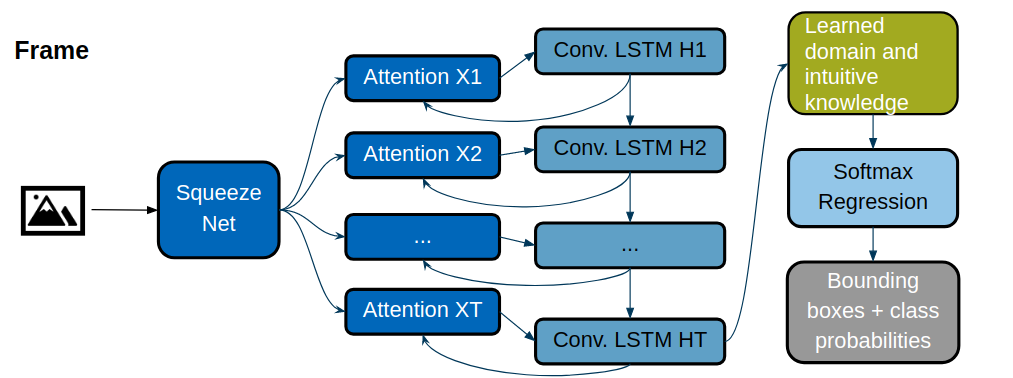
\includegraphics[width=\columnwidth]{KB-RANN-architecture}
\begin{itemize}
	\item Compute feature maps using a modified SqueezeNet architecture.
	\item Propagate the features through a Recurrent Attentive Neural Network, comprised of:
	\begin{itemize}
		\item Attention Mechanism to detect key areas within the feature maps.
		\item Convolutional LSTM for temporal feature propagation.	
	\end{itemize}
	\item Reverse gaussian feature maps are combined with the maps obtained from Conv. LSTM.
	\begin{itemize}
		\item These feature maps are based on learnable mean and covariance terms.
		\item This prior knowledge is derived from the assumption that traffic signs are always located at the bias of the center.

	\end{itemize}
\end{itemize}

\subsection{Looking fast and slow: memory-guided mobile video object detection}
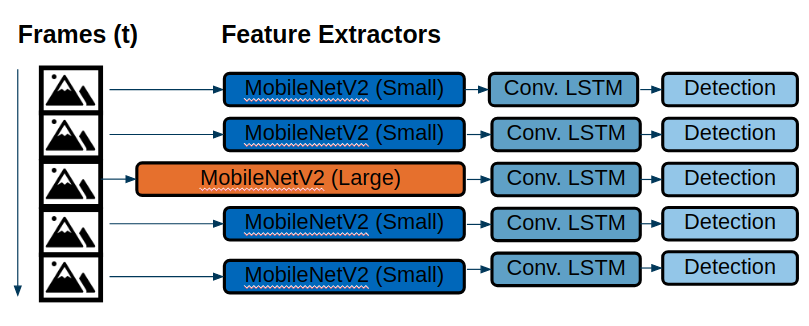
\includegraphics[width=\columnwidth]{looking-fast-and-slow-architecture}
\begin{itemize}
	\item Run multiple feature extractors sequentially or concurrently to obtain feature maps.
	\begin{itemize}
		\item 	The idea is to use small and large feature extractors to optimize performance.
	\end{itemize}
	\item Aggregate and refine these feature maps using convolutional LSTM based memory network.
	\begin{itemize}
		\item To improve speed of LSTM network, add skip connections and LSTM state groups.
	\end{itemize}
	\item Apply SSD-style detection on refined features to obtain classification and bounding boxes.
	\item Use a reinforcement learning based policy for selection of which feature extractor to run.
	\item Large and small frame extractors can run in parallel using asynchronous mode.
\end{itemize}

\subsection{Detect to Track and track to detect}
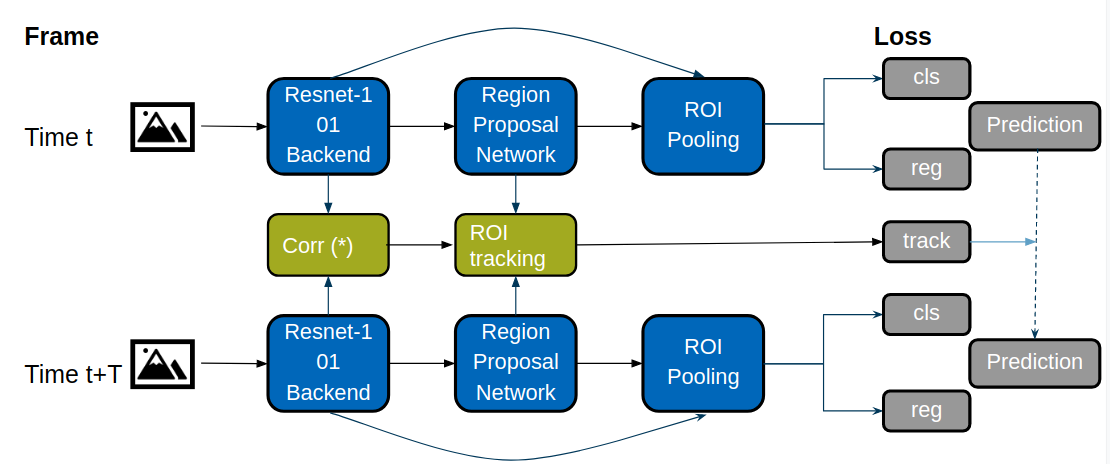
\includegraphics[width=\columnwidth]{D&T-architecture}
\begin{itemize}
	\item Compute Convolutional feature maps using a Resnet-101 architecture.
	\item Use a RPN (region proposal network) to find candidate regions in the frame.
	\item ROI Pooling layer, to classify boxes and refine their coordinates (regression).
	\item Find correlation features between two frames’ feature maps and do ROI tracking.
	\item Due to memory constraints, use tracklets, which are class-based optimal paths in video.

\end{itemize}

\section{Box-Level-based Video Object Detection}

\subsection{Definition}
ToDo

\subsection{Object Detection from Video Tubelets with Convolutional Neural Networks}
ToDo

\subsection{Optimizing Video Object Detection via Scale-Time Lattice}
ToDo

\subsection{Context Matters: Refining Object Detection in Video with Recurrent Neural Networks}
ToDo

\subsection{Spatially Supervised Recurrent Convolutional Neural Networks for Visual Object Tracking}
ToDo


\section{Flow-based Object Detection}

\subsection{Definition}
Todo

\subsection{Deep Feature Flow for Video Recognition}
Todo

\section{Comparison of different approaches}

\subsection{General}
ToDo

\subsection{Conclusion Perfomance}
Todo

\subsection{Conclusion Prediction Quality}
Todo


\section{Outro}

\subsection{Conclusion}
Todo

\subsection{Further work}
Todo


\section*{Acknowledgment}
Todo

\section*{References}

Please number citations consecutively within brackets \cite{b1}. The 
sentence punctuation follows the bracket \cite{b2}. Refer simply to the reference 
number, as in \cite{b3}---do not use ``Ref. \cite{b3}'' or ``reference \cite{b3}'' except at 
the beginning of a sentence: ``Reference \cite{b3} was the first $\ldots$''

Number footnotes separately in superscripts. Place the actual footnote at 
the bottom of the column in which it was cited. Do not put footnotes in the 
abstract or reference list. Use letters for table footnotes.

Unless there are six authors or more give all authors' names; do not use 
``et al.''. Papers that have not been published, even if they have been 
submitted for publication, should be cited as ``unpublished'' \cite{b4}. Papers 
that have been accepted for publication should be cited as ``in press'' \cite{b5}. 
Capitalize only the first word in a paper title, except for proper nouns and 
element symbols.

For papers published in translation journals, please give the English 
citation first, followed by the original foreign-language citation \cite{b6}.

\begin{thebibliography}{00}
\bibitem{b1} G. Eason, B. Noble, and I. N. Sneddon, ``On certain integrals of Lipschitz-Hankel type involving products of Bessel functions,'' Phil. Trans. Roy. Soc. London, vol. A247, pp. 529--551, April 1955.
\bibitem{b2} J. Clerk Maxwell, A Treatise on Electricity and Magnetism, 3rd ed., vol. 2. Oxford: Clarendon, 1892, pp.68--73.
\bibitem{b3} I. S. Jacobs and C. P. Bean, ``Fine particles, thin films and exchange anisotropy,'' in Magnetism, vol. III, G. T. Rado and H. Suhl, Eds. New York: Academic, 1963, pp. 271--350.
\bibitem{b4} K. Elissa, ``Title of paper if known,'' unpublished.
\bibitem{b5} R. Nicole, ``Title of paper with only first word capitalized,'' J. Name Stand. Abbrev., in press.
\bibitem{b6} Y. Yorozu, M. Hirano, K. Oka, and Y. Tagawa, ``Electron spectroscopy studies on magneto-optical media and plastic substrate interface,'' IEEE Transl. J. Magn. Japan, vol. 2, pp. 740--741, August 1987 [Digests 9th Annual Conf. Magnetics Japan, p. 301, 1982].
\bibitem{b7} M. Young, The Technical Writer's Handbook. Mill Valley, CA: University Science, 1989.
\end{thebibliography}
\vspace{12pt}
\color{red}
IEEE conference templates contain guidance text for composing and formatting conference papers. Please ensure that all template text is removed from your conference paper prior to submission to the conference. Failure to remove the template text from your paper may result in your paper not being published.

\end{document}
